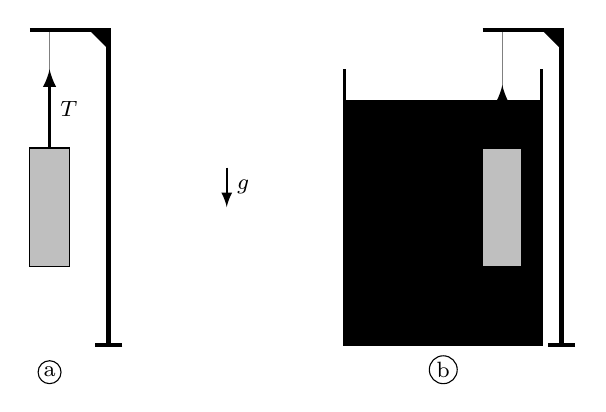
\begin{tikzpicture} [
	scale=0.5,
	font=\footnotesize,
	vecteur/.style={-latex,thick},
	force/.style={->,>=latex,draw=\JRLblue,very thick,nodes={\JRLblue}},
	liquide/.style={fill=\JRLblueC,very thin,draw=\JRLblueF},
    solide/.style={fill=lightgray},
	]
	% \draw[help lines] (0,0) grid (10,10);
	\draw[solide,shift={(0,2)}] (0,0)rectangle(1,3);
	\draw[thin,gray,shift={(0,2)}] (.5,3)--++(0,3);
	\draw[ultra thick,shift={(0,2)}] (0,6)-|(2,-2)++(10pt,0)--++(-20pt,0);
	\fill[shift={(2,8)}](0,-.5)|-(-.5,0)--cycle;
	\node[draw,circle,inner sep=1pt] at (0.5,-1) [above]{a};
	\draw[vecteur,shift={(5,4)}] (0,0.5)--(0,-0.5)node[right,midway]{$\vv{g}$};
	\draw[force,shift={(0,2)}] (0.5,3)--++(0,2)node[right,midway]{$\vv{T}$};
	\begin{scope}[shift={(10.5,0)}]
%		\shadedraw[color=gray,top color=white,bottom color=gray] (-2.5,6.2)--++(0,-6.2)--++(5,0)--++(0,6.2)--cycle;
		\draw[liquide] (-2.5,6.2)--++(0,-6.2)--++(5,0)--++(0,6.2)--cycle;
		\draw[line width=1pt] (-2.5,7)--++(0,-7)--++(5,0)--++(0,7);
		\draw(0,1) node[above]{eau ($\rho_\text{e}$)};
		\draw[solide,shift={(1,2)}] (0,0)rectangle(1,3);
		\draw[thin,gray,shift={(1,2)}] (.5,3)--++(0,3);
		\draw[ultra thick,shift={(1,2)}] (0,6)-|(2,-2)++(10pt,0)--++(-20pt,0);
		\fill[shift={(3,8)}](0,-.5)|-(-.5,0)--cycle;
		\draw[force,shift={(1,2)}] (0.5,3)--++(0,1.6)node[right,midway]{$\vv{T'}$};
		\node[draw,circle,inner sep=1pt] at (0,-1) [above]{b};
	\end{scope}
\end{tikzpicture}